\chapter{Elements of SDLC}

\section{SDLC Methodology}

The Software Development Life Cycle (SDLC) for this project followed a hybrid approach, combining the structured framework of the Waterfall model with Agile elements for flexibility. While Waterfall provided sequential stages (requirement analysis, design, implementation, testing), Agile practices like ongoing feedback and peer-reviewed GitHub pull requests (PRs) were integrated. This PR review process allowed team members to assess code, identify issues early, and ensure quality and consistency. This hybrid methodology balanced systematic progression with iterative refinement based on team collaboration and insights.

\section{Gantt Chart}

% Force proper figure numbering once before the figure
\renewcommand{\thefigure}{3.\arabic{figure}}

% Full page figure with rotated image on a separate page
\begin{figure}[p]
    \centering
    % Rotate the image 90 degrees 
    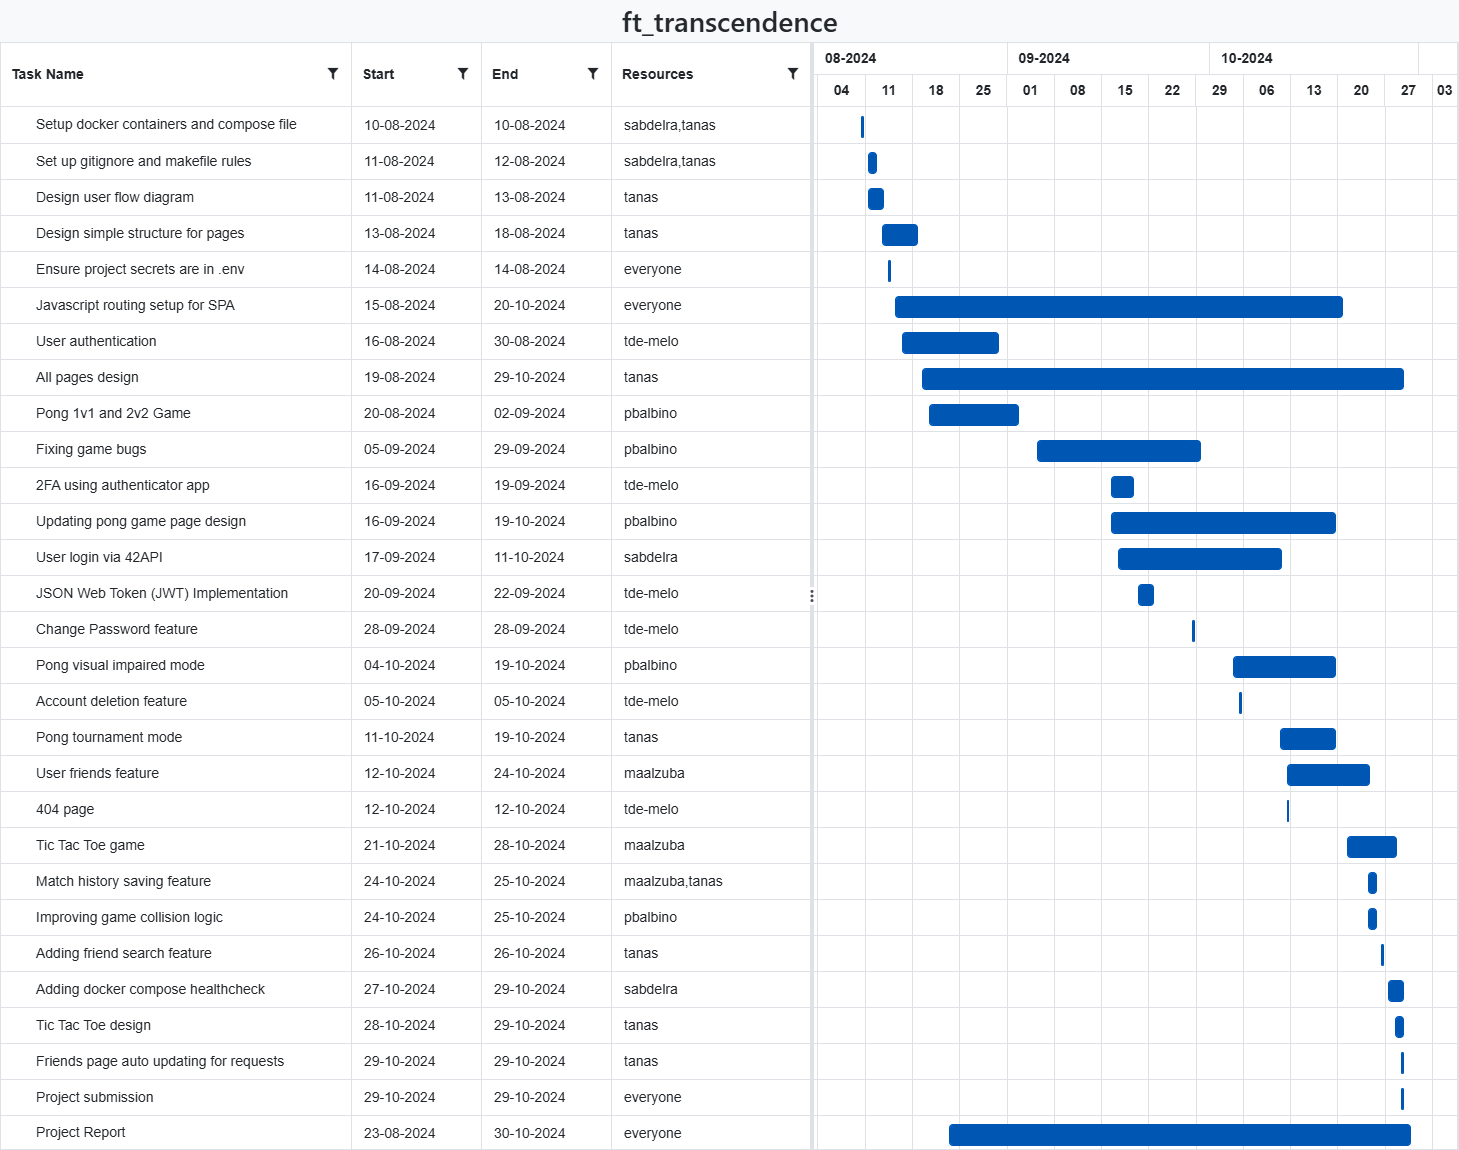
\includegraphics[angle=90, width=1\textwidth, height=1\textheight, keepaspectratio]{Figures/images/gantt-chart.png}
    \caption{Gantt Chart}
    \label{fig:gantt-chart}
\end{figure}


\clearpage
% Begin explanatory text on a new page
The Gantt Chart (Figure \ref{fig:gantt-chart}) delineates the project timeline, outlining tasks, dependencies, and milestones, thereby mapping the project's progression through each phase of the Software Development Life Cycle (SDLC).

This Gantt chart outlines the project timeline for \textbf{ft\_transcendence}, showing tasks, their durations, and assigned resources. It spans from February to May 2025, covering development milestones like setting up the \textbf{Docker environment} with \textbf{Docker-Compose}, designing user interfaces using \textbf{Bootstrap 5}, and implementing essential features such as user authentication (\textbf{Native Credentials, 42 OAuth, JWT, TOTP 2FA}). The project includes building the main Pong game modes (\textbf{1v1, vs AI, 4-player local, Tournaments}), integrating \textbf{Blockchain} for tournament storage, setting up the \textbf{ELK stack} for monitoring, and implementing user features like friend management, match history, and account settings. Key phases involved requirements analysis, design, implementation, testing, debugging, and documentation updates, with the final submission completed by May 1st, 2025. Various team members were responsible for specific tasks, ensuring collaborative progress throughout the development period.

\section{Risk Assessment and Management}

\subsection{Risk Assessment Methodology}
The risk assessment process for the ft\_transcendence project involved identifying potential risks, evaluating their likelihood and impact, and developing mitigation strategies. This systematic approach ensured that potential threats to project success were proactively managed throughout the development lifecycle. Risks were evaluated using the following scales:

\begin{table}[H]
    \centering
    \renewcommand{\arraystretch}{1.5}
    \begin{tabular}{|c|p{12cm}|}
    \hline
    \textbf{Impact Level} & \textbf{Description} \\
    \hline
    1 - Insignificant & Minimal impact on functionality or project timeline \\
    \hline
    2 - Minor & Minor impact on specific features, easily recoverable \\
    \hline
    3 - Moderate & Noticeable impact on major features, requires significant effort to resolve \\
    \hline
    4 - Major & Serious impact on core functionality or security, could compromise project success \\
    \hline
    5 - Severe & Critical system failure or security breach, potentially unrecoverable \\
    \hline
    \end{tabular}
    \caption{Impact Scale for Risk Assessment}
    \label{tab:impact_scale}
\end{table}

\begin{table}[H]
    \centering
    \renewcommand{\arraystretch}{1.5}
    \begin{tabular}{|c|p{12cm}|}
    \hline
    \textbf{Likelihood Level} & \textbf{Description} \\
    \hline
    1 - Rare & Highly unlikely to occur during the project lifecycle \\
    \hline
    2 - Unlikely & Could occur but probability remains low \\
    \hline
    3 - Possible & May occur during the project lifecycle \\
    \hline
    4 - Likely & Will probably occur under current project conditions \\
    \hline
    5 - Almost Certain & Expected to occur multiple times during the project lifecycle \\
    \hline
    \end{tabular}
    \caption{Likelihood Scale for Risk Assessment}
    \label{tab:likelihood_scale}
\end{table}

\subsection{Risk Matrix}
The risk matrix provides a visual representation of the severity of identified risks based on their likelihood and potential impact. This visualization aids in prioritizing mitigation efforts for the most critical risks.

\begin{table}[H]
    \centering
    \renewcommand{\arraystretch}{2} % Increase the height of each cell
    \begin{tabular}{c|c|c|c|c|c|c|}
    \multicolumn{1}{c}{} & \multicolumn{5}{c}{\textbf{Impact}} \\
    \cline{2-7}
    \multicolumn{1}{c|}{} & \textbf{Risk Matrix} & \textbf{Insignificant 1} & \textbf{Minor 2} & \textbf{Moderate 3} & \textbf{Major 4} & \textbf{Severe 5} \\
    \hline
    \multirow{5}{*}{\rotatebox{90}{\textbf{Likelihood}}} 
    & \textbf{Almost Certain 5} & \cellcolor{yellow!50}Medium 5 & \cellcolor{orange!50}High 10 & \cellcolor{red!50}Very High 15 & \cellcolor{red!70}Extreme 20 & \cellcolor{red!70}Extreme 25 \\
    \cline{2-7}
    & \textbf{Likely 4} & \cellcolor{yellow!50}Medium 4 & \cellcolor{yellow!50}Medium 8 & \cellcolor{orange!50}High 12 & \cellcolor{red!50}Very High 16 & \cellcolor{red!70}Extreme 20 \\
    \cline{2-7}
    & \textbf{Possible 3} & \cellcolor{green!100}Low 3 & \cellcolor{yellow!50}Medium 6 & \cellcolor{yellow!50}Medium 9 & \cellcolor{orange!50}High 12 & \cellcolor{red!50}Very High 15 \\
    \cline{2-7}
    & \textbf{Unlikely 2} & \cellcolor{green!50}Very Low 2 & \cellcolor{green!100}Low 4 & \cellcolor{yellow!50}Medium 6 & \cellcolor{yellow!50}Medium 8 & \cellcolor{orange!50}High 10 \\
    \cline{2-7}
    & \textbf{Rare 1} & \cellcolor{green!50}Very Low 1 & \cellcolor{green!50}Very Low 2 & \cellcolor{green!100}Low 3 & \cellcolor{yellow!50}Medium 4 & \cellcolor{yellow!50}Medium 5 \\
    \hline
    \end{tabular}
    \caption{Risk Matrix}
    \label{tab:risk_matrix}
\end{table}

The status of each risk was monitored continuously throughout the project's duration to ensure timely responses. To facilitate the analysis and mitigation process, the risks were divided between the \textit{Frontend Team} and the \textit{Backend Team}, considering the project's scope and the number of developers involved.

\subsection{Risk Register}
The following register documents the specific risks identified for the ft\_transcendence project, along with their assessed impact, likelihood, severity, and mitigation strategies.

\begin{table}[H]
    \footnotesize
    \centering
    \renewcommand{\arraystretch}{1.2} % Slightly compact rows
    \begin{tabular}{|p{3.2cm}|c|c|c|p{1.5cm}|p{5cm}|}
    \hline
    \textbf{Risk Description} & \textbf{Impact} & \textbf{Like.} & \textbf{Sev.} & \textbf{Owner} & \textbf{Mitigation Strategy} \\
    \hline
    \multicolumn{6}{|c|}{\textbf{Impact}: 1-Low to 5-High, \textbf{Likelihood}: 1-Low to 5-High, \textbf{Severity}: Impact × Likelihood} \\
    \hline
    Security vulnerabilities in JWT implementation & 5 & 2 & 10 & Backend & Implement proper JWT validation, secure storage of secrets, follow security best practices \\
    \hline
    2FA setup/validation issues causing login failures & 4 & 2 & 8 & Backend & Test 2FA flows thoroughly, implement recovery options, provide clear user guidance \\
    \hline
    42 OAuth integration failure affecting authentication & 4 & 3 & 12 & Backend & Create fallback auth methods, ensure error handling, maintain OAuth documentation \\
    \hline
    Canvas rendering performance problems & 3 & 4 & 12 & Frontend & Optimize game loop, implement frame rate limiting, test on various devices \\
    \hline
    Blockchain integration failures & 3 & 3 & 9 & Backend & Implement transaction queuing, retry mechanisms, fallback PostgreSQL records \\
    \hline
    Docker container privilege escalation vulnerabilities & 5 & 2 & 10 & DevOps & Run services as non-root users, implement proper volume permissions, keep images updated \\
    \hline
    Database connection pool exhaustion & 4 & 2 & 8 & Backend & Configure connection pool limits, implement recycling, monitor DB performance \\
    \hline
    NGINX configuration issues affecting functionality & 4 & 2 & 8 & DevOps & Test configurations thoroughly, automate certificate renewal, implement health checks \\
    \hline
    Game logic bugs affecting match fairness & 3 & 3 & 9 & Frontend & Implement unit tests for game logic, test edge cases, validate game state consistently \\
    \hline
    Frontend responsiveness issues for mobile/tablet & 3 & 3 & 9 & Frontend & Test across screen sizes, implement responsive design, use Bootstrap grid properly \\
    \hline
    ELK stack configuration issues & 2 & 2 & 4 & DevOps & Validate logging pipeline, implement structured logging format, monitor log volume \\
    \hline
    PostgreSQL data loss during tournament play & 4 & 1 & 4 & Backend & Implement regular backups, validate data integrity, use proper transaction management \\
    \hline
    High latency affecting multiplayer experience & 4 & 4 & 16 & Frontend & Implement client-side prediction, optimize network payload, provide visual feedback \\
    \hline
    Cross-browser compatibility issues & 3 & 2 & 6 & Frontend & Test on major browsers, implement feature detection, provide graceful fallbacks \\
    \hline
    \end{tabular}
    \caption{Risk Register}
    \label{tab:risk_register}
\end{table}

\subsection{High Priority Risks}
Based on the risk matrix analysis, the following risks were identified as high priority (severity score $\geq 12$) and required immediate attention and proactive mitigation:

\begin{enumerate}
    \item \textbf{High latency affecting multiplayer game experience (16):} The real-time nature of Pong makes it particularly susceptible to latency issues. The team implemented client-side prediction techniques to smooth gameplay even when network conditions were suboptimal. Additionally, network packet size was optimized to minimize transmission delays.
    

    \item \textbf{42 OAuth integration failure (12):} As a key authentication mechanism, issues with the 42 OAuth integration could severely impact user access. Comprehensive error handling was implemented along with detailed logs to quickly identify and address integration issues.
    
    \item \textbf{Canvas rendering performance problems (12):} Performance optimization techniques were applied to ensure smooth gameplay across a range of devices. This included implementing a consistent frame rate cap and optimizing render cycles.
\end{enumerate}

\subsection{Risk Monitoring and Control}
Throughout the project lifecycle, risks were continuously monitored and reassessed. The development team implemented the following control measures:

\begin{itemize}
    \item \textbf{Weekly risk reviews} during team meetings to update risk status and mitigation effectiveness
    \item \textbf{Automated testing} to detect issues early in the development process
    \item \textbf{Performance monitoring} using the ELK stack to identify potential problems before they affected users
    \item \textbf{Security scanning} of dependencies and Docker containers to identify new vulnerabilities
    \item \textbf{User feedback collection} during testing phases to identify UX issues
\end{itemize}

\section{Functional Requirements}
\subsection*{User Authentication and Management}
\begin{itemize}
    \item Secure registration, login, and profile management.
    \item Support for multiple authentication mechanisms: Native username/password, 42 Intra OAuth 2.0, and optional TOTP-based Two-Factor Authentication (2FA).
    \item User profile management features, including unique display names, avatar uploads, and online status visibility.
    \item Friends list management (add, remove, view status).
\end{itemize}


\subsection*{Gameplay and Game Modes}
\begin{itemize}
    \item Core Pong gameplay implemented on HTML5 Canvas.
    \item Multiple game modes:
        \begin{itemize}
            \item 1 vs 1: Online match against another registered user.
            \item 1 vs AI: Match against a computer-controlled opponent.
            \item Local Multiplayer: Up to 4 players on the same screen.
            \item Tournament: Knockout bracket competition among registered users.
        \end{itemize}
\end{itemize}

\subsection*{Match History and Statistics}
\begin{itemize}
    \item Tracking and storing user gameplay statistics, including wins, losses.
    \item Displaying match history for logged-in users.
    \item Recording tournament results in PostgreSQL and immutably on the Ethereum sidechain.
\end{itemize}

\subsection*{Accessibility Features}
\begin{itemize}
    \item Considerations for visually impaired users (e.g., high-contrast options, clear UI elements).
    \item Keyboard navigation support for gameplay and interface interaction.
\end{itemize}

\section{Technical Requirements}
\section*{Software Specifications}

\subsection*{Operating System}
\begin{itemize}
    \item \textbf{Server Deployment}: Linux-based distribution (e.g., Debian, Ubuntu) is recommended for hosting Docker containers.
    \item \textbf{Development/Client}: Cross-platform compatibility (Linux, macOS, Windows) for development and playing via supported web browsers.
\end{itemize}

\subsection*{Programming Languages, Frameworks, and Libraries}
\begin{itemize}
    \item \textbf{Backend}: Python 3 with Django 5 framework. Django Rest Framework (DRF) for API development. Libraries include `djangorestframework-simplejwt` for JWT authentication and `django-otp` for 2FA.
    \item \textbf{Frontend}: Vanilla JavaScript (ES6+), HTML5, CSS3. Bootstrap 5 for responsive UI components and layout.
    \item \textbf{Blockchain Interaction}: Web3.py library for interacting with the Ethereum sidechain from the backend (or helper scripts).
\end{itemize}

\subsection*{Database and Data Storage}
\begin{itemize}
    \item \textbf{Primary Database}: PostgreSQL (Version 15 specified) for storing user data, match history, game settings, etc.
    \item \textbf{Blockchain}: Local Ethereum Proof-of-Authority (POA) sidechain (using Geth) for immutable storage of tournament results. Smart contracts developed in Solidity (details likely in `Blockchain/` directory).
\end{itemize}

\subsection*{Web Server and Reverse Proxy}
\begin{itemize}
    \item Nginx: Used as a reverse proxy to route traffic to the Django backend (via Gunicorn or similar WSGI server), serve static frontend files (JS, CSS, images), and handle TLS/SSL termination for HTTPS.
\end{itemize}

\subsection*{Containerization and Orchestration}
\begin{itemize}
    \item Docker: To containerize each service (frontend, backend, database, Nginx, ELK, blockchain node).
    \item Docker-Compose: To define and manage the multi-container application stack.
\end{itemize}

\subsection*{Authentication and Security Mechanisms}
\begin{itemize}
    \item JSON Web Tokens (JWT): Used for stateless session management via secure HTTP-only cookies.
    \item Two-Factor Authentication (2FA): TOTP-based 2FA support via `django-otp`.
    \item OAuth 2.0: Integration with 42 Intra's OAuth service.
    \item TLS/SSL: Encryption for all communication via HTTPS, handled by Nginx.
\end{itemize}

\subsection*{Monitoring and Logging}
\begin{itemize}
    \item ELK Stack: Elasticsearch (Version 7 specified) for log aggregation and indexing, Kibana (Version 8 specified) for visualization and analysis. Log shipping likely handled by Filebeat or integrated Django logging.
\end{itemize}

\section*{Hardware Specifications}
\subsection*{Server Requirements (Development/Small Scale)}
\begin{itemize}
    \item Processor: Modern multi-core CPU.
    \item Memory: Minimum 8 GB RAM (16 GB+ recommended, especially with ELK stack).
    \item Storage: SSD recommended (minimum 50-100 GB, depending on data volume and logs).
    \item Network: Standard internet connectivity.
\end{itemize}
*Note: Production requirements would depend heavily on user load.*

\subsection*{Client Requirements}
\begin{itemize}
    \item Device: Desktop, laptop with modern web browser.
    \item Browser: Latest versions of Chrome or Firefox recommended.
    \item Network: Stable internet connection for real-time gameplay.
\end{itemize}

\section*{System Architecture}
\subsection*{Client Layer (Frontend SPA)}
The frontend is a Single-Page Application (SPA) responsible for rendering the user interface, handling user interactions, and managing client-side game logic. Technologies:
\begin{itemize}
    \item Framework/Libraries: Vanilla JavaScript (ES6+), Bootstrap 5.
    \item Structure: HTML templates, CSS3 for styling.
    \item Rendering: Client-side rendering. Game logic executed directly in the browser, primarily using the HTML5 Canvas API for Pong gameplay.
    \item API Communication: Uses Fetch API or similar to interact with the backend REST API for data retrieval, user actions, and submitting game results.
    \item Authentication Handling: Manages JWT tokens received from the backend (stored securely, likely in HttpOnly cookies handled by the browser).
\end{itemize}

\subsection*{Application Layer (Backend API)}
The backend provides the RESTful API, manages business logic, handles user authentication, interacts with the database and blockchain, and integrates with monitoring systems. Technologies:
\begin{itemize}
    \item Framework: Django 5 (Python 3).
    \item API: Django Rest Framework (DRF) for creating API endpoints.
    \item Authentication: Handles user registration, login (native, OAuth), JWT generation/validation (`djangorestframework-simplejwt`), and 2FA logic (`django-otp`).
    \item Database Interaction: Uses Django ORM to communicate with the PostgreSQL database.
    \item Blockchain Interaction: May trigger helper scripts (`Web3.py`) to interact with the Ethereum sidechain for storing tournament data.
    \item Logging: Integrates with the ELK stack for centralized logging.
    \item WSGI Server: Typically runs behind Nginx using a WSGI server like Gunicorn (though not explicitly mentioned in README, it's standard for Django deployment).
\end{itemize}

\subsection*{Data Layer (Persistence)}
The data layer ensures persistent storage of application data using both relational and blockchain technologies. Technologies:
\begin{itemize}
    \item Relational Database: PostgreSQL 15 for user accounts, profiles, settings, individual match history, etc.
    \item Blockchain Database: Ethereum sidechain (Geth node running POA) for immutable recording of official tournament outcomes via smart contracts.
\end{itemize}

\subsection*{Infrastructure Layer (Orchestration and Hosting)}
This layer encompasses the tools and services used for deployment, management, and operation of the application stack. Technologies:
\begin{itemize}
    \item Containerization: Docker packages each component (frontend, backend, Postgres, Nginx, ELK, Geth) into isolated containers.
    \item Orchestration: Docker-Compose defines the relationships and configurations for running the multi-container application.
    \item Reverse Proxy / Web Server: Nginx manages incoming HTTPS traffic, routes requests to the appropriate backend service, serves static frontend assets, and handles SSL/TLS termination.
    \item Monitoring: ELK Stack (Elasticsearch, Kibana) provides infrastructure for log aggregation and analysis.
\end{itemize}

\subsection*{Communication and Networking}
\begin{itemize}
    \item Internal Communication: Services within the Docker network communicate over a private network defined by Docker-Compose.
    \item External Communication: All external client communication occurs over HTTPS (port 443), managed by Nginx.
    \item API Calls: Frontend communicates with the backend via RESTful HTTP requests to the API endpoints.
    \item Blockchain Calls: Backend (or scripts triggered by it) communicates with the Geth node via RPC calls (typically over HTTP or IPC).
\end{itemize}

\section{Non-functional Requirements}
Non-functional requirements define the quality attributes and constraints of the system.

\subsection*{Performance}
\begin{itemize}
    \item \textbf{Responsiveness}: The SPA frontend should provide a smooth user experience with minimal delays during navigation and interaction. Game rendering on the Canvas should be efficient to maintain playable frame rates.
    \item \textbf{Latency}: Network latency for real-time 1v1 games should be minimized, although the current implementation seems focused on client-side rendering with results submitted post-game. API response times should be reasonably fast.
    \item \textbf{Load Handling}: The system (especially Nginx and the Django backend) should be capable of handling a moderate number of concurrent users, scalable via Docker if needed.
\end{itemize}

\subsection*{Security}
\begin{itemize}
    \item \textbf{Authentication}: Secure mechanisms for login (native, 42 OAuth) and session management (JWT over HTTPS, HttpOnly cookies).
    \item \textbf{Authorization}: Proper checks to ensure users can only access their own data and perform actions they are permitted to.
    \item \textbf{Data Protection}: Use of HTTPS (TLS/SSL) for all external communication. Sensitive data in the database should be handled securely (e.g., password hashing via Django). Input validation to prevent common web vulnerabilities (XSS, SQL Injection) provided by Django/DRF.
    \item \textbf{Infrastructure Security}: Containers should run with non-root users. Network policies within Docker can restrict communication between containers.
    \item \textbf{2FA}: Optional TOTP-based 2FA provides an additional security layer.
\end{itemize}

\subsection*{Reliability}
\begin{itemize}
    \item \textbf{Availability}: The application should be available with minimal downtime. Docker and Nginx help manage service availability.
    \item \textbf{Data Integrity}: PostgreSQL ensures relational data integrity. Blockchain provides immutability for tournament records.
    \item \textbf{Fault Tolerance}: Containerized architecture allows individual services to be restarted if they fail. Error handling should be robust in both frontend and backend.
    \item \textbf{Backup and Recovery}: Regular backups of the PostgreSQL database are crucial (mentioned as a mitigation strategy).
\end{itemize}

\subsection*{Scalability}
\begin{itemize}
    \item \textbf{Component Scaling}: Docker-Compose allows scaling individual services (e.g., adding more backend instances) if necessary, although load balancing setup might need adjustment.
    \item \textbf{Database Scaling}: PostgreSQL offers various scaling options if needed in the future.
    \item \textbf{Stateless Backend}: Using JWT promotes a stateless backend architecture, which generally scales better horizontally.
\end{itemize}

\subsection*{Maintainability}
\begin{itemize}
    \item \textbf{Modularity}: The project is divided into distinct components (Frontend, Backend, Blockchain, Infrastructure) and containerized services, promoting separation of concerns.
    \item \textbf{Code Quality}: Adherence to coding standards and use of frameworks (Django, Bootstrap) aids maintainability.
    \item \textbf{Configuration Management}: Environment variables (`.env` file) are used for configuration, separating code from configuration.
    \item \textbf{DevOps Automation}: Makefile and Docker-Compose simplify build, deployment, and management tasks.
\end{itemize}

\subsection*{Usability and Accessibility}
\begin{itemize}
    \item \textbf{User Interface}: The UI, built with Bootstrap, should be intuitive and easy to navigate.
    \item \textbf{Responsiveness}: The application should adapt to different screen sizes (desktops primarily, given the game type).
    \item \textbf{Accessibility}: Conscious effort to include features for visually impaired users (high contrast, keyboard navigation) as stated in goals.
\end{itemize}

\section{Implementation}
The implementation phase involved developing the actual code and functionality based on the design specifications. Key aspects included:
\begin{itemize}
    \item \textbf{Backend Development:} Core functionality was built using Django and Django Rest Framework (DRF), providing a secure RESTful API. This included managing user data (PostgreSQL), handling authentication (Native, 42 OAuth, JWT, 2FA), supporting multiple Pong game modes, and ensuring security against common vulnerabilities like SQL injection and XSS through Django's built-in features.
    \item \textbf{Frontend Development:} A responsive Single-Page Application (SPA) interface was built using Vanilla JavaScript, HTML5, and CSS3, leveraging Bootstrap 5 for layout and components. Accessibility features like high-contrast themes and keyboard navigation were incorporated. The frontend interacts with the backend API and uses the HTML5 Canvas for rendering the Pong game dynamically.
    \item \textbf{Game Development:} Pong game mechanics were implemented using JavaScript and Canvas, including ball/paddle physics, scoring, and real-time updates. Game modes (1v1, vs AI, 4-player local, Tournament) were developed.
    \item \textbf{Blockchain Integration:} Smart contracts (Solidity) were developed and deployed to a local Ethereum sidechain (Geth) to immutably record tournament results. Backend interaction was handled using Web3.py.
    \item \textbf{User History and Statistics:} A system was integrated to track and display user match history and statistics (wins/losses), stored primarily in PostgreSQL.
    \item \textbf{User Management and Authentication:} Secure user registration, login (Native, 42 OAuth), profile management (display name, avatar), friends list, and TOTP 2FA were implemented. JWTs, managed via secure HttpOnly cookies, were used for session management.
    \item \textbf{DevOps and Deployment:} The entire application (Backend, Frontend, PostgreSQL, Nginx, ELK, Geth node) was containerized using Docker and orchestrated with Docker Compose. Nginx served as a reverse proxy and static file server. The ELK stack was configured for centralized logging and monitoring.
    \item \textbf{Collaborative Workflow:} GitHub branches were used for parallel development (e.g., backend, frontend, game features). Peer reviews were conducted on Pull Requests before merging to the main branch to maintain code quality.
\end{itemize}

\section{Testing}
The testing phase ensured the application's functionality, security, usability, and adherence to requirements. Key testing types included:
\begin{itemize}
    \item \textbf{Unit Testing:} Verifying individual components like authentication logic, specific API endpoints, Canvas rendering functions, and game rule implementations (e.g., ball collision, scoring) in isolation.
    \item \textbf{Integration Testing:} Testing interactions between components, such as frontend API calls to the backend for login/registration, fetching user profiles, submitting game results, database interactions (PostgreSQL CRUD operations), and backend communication with the Ethereum sidechain.
    \item \textbf{Functional Testing:} Validating end-to-end features against requirements. This involved testing all Pong game modes, user registration/login flows (Native, OAuth, 2FA), profile updates, friend management, tournament creation/participation, and ensuring restricted content access controls worked correctly.
    \item \textbf{Usability Testing:} Evaluating the user interface and experience for intuitiveness and accessibility. Testing responsiveness across different screen sizes (desktop, tablet, mobile) using Bootstrap, checking keyboard navigation, and verifying accessibility features for visually impaired users.
    \item \textbf{Compatibility Testing:} Ensuring consistent functionality across target browsers (latest Chrome and Firefox).
    \item \textbf{Security Testing:} Reviewing implementations for common web vulnerabilities (though specific penetration testing might not have been performed), verifying JWT handling, 2FA enforcement, and general adherence to security best practices mentioned in mitigation strategies.
    \item \textbf{CI/CD Integration:} Using GitHub Actions to automate checks (e.g., linters, basic tests) to prevent merging failing code into the main branch.
\end{itemize}

\section{Evolution}
This phase focuses on maintaining and enhancing the software post-initial deployment.
\subsection*{Backend Development}
\begin{itemize}
    \item \textbf{Initial Phase:} Focused on core Django/DRF setup, basic user auth, and foundational API endpoints for Pong.
    \item \textbf{Intermediate Phase:} Expanded to support multiple game modes, integrated 42 OAuth and 2FA, developed blockchain interaction logic (Web3.py), and refined APIs based on frontend needs.
    \item \textbf{Current Phase:} Provides a comprehensive API managing users, game logic, statistics, tournaments (with blockchain logging), and authentication, running within a Dockerized environment integrated with ELK.
\end{itemize}

\subsection*{Frontend Development}
\begin{itemize}
    \item \textbf{Initial Phase:} Basic SPA structure with Vanilla JS, Bootstrap layout, initial Canvas implementation for Pong.
    \item \textbf{Intermediate Phase:} Refined UI/UX based on feedback, improved responsiveness, enhanced Canvas rendering, integrated API calls for dynamic data, added accessibility features.
    \item \textbf{Current Phase:} Delivers an interactive SPA experience with real-time updates, customizable settings, smooth navigation, robust game interface via Canvas, and accessibility considerations.
\end{itemize}

\subsection*{Game Development}
\begin{itemize}
    \item \textbf{Initial Phase:} Developed core Pong mechanics on Canvas (ball/paddle movement, collision, scoring).
    \item \textbf{Intermediate Phase:} Added different game modes (1v1, AI, 4-player, Tournament), improved real-time responsiveness, added basic customization.
    \item \textbf{Current Phase:} Offers multiple Pong game modes integrated seamlessly within the SPA, with results feeding into the user history and tournament system.
\end{itemize}

\subsection*{User History and Statistics}
\begin{itemize}
    \item \textbf{Initial Phase:} Basic recording of game outcomes to PostgreSQL.
    \item \textbf{Intermediate Phase:} Expanded tracking to include more details (opponents, scores, dates), developed API endpoints for retrieval.
    \item \textbf{Current Phase:} Provides comprehensive user statistics and match history accessible via the user profile, with tournament results also logged immutably on the blockchain.
\end{itemize}

\subsection*{User Management and Authentication}
\begin{itemize}
    \item \textbf{Initial Phase:} Implemented native registration/login, basic profile management.
    \item \textbf{Intermediate Phase:} Added 42 OAuth integration, JWT implementation, friend list functionality, and initial 2FA setup.
    \item \textbf{Current Phase:} Offers a robust system with multiple auth methods (Native, OAuth, 2FA), secure session management (JWT via HttpOnly cookies), comprehensive profile features (avatar, stats), and friend management.
\end{itemize}